\appendix

\chapter{Installation Guides}

To work through this tutorial requires to have a working installation
of MOLE.
It relies on
\href{https://gitlab.com/conradsnicta/armadillo-code}{\mintinline{cpp}|armadillo|}~\cite{Sanderson2025},
a C++ library that provides data structures for sparse matrices.
We explain the step-by-step process for
\href{https://wiki.archlinux.org/title/Pacman/Rosetta}{Arch Linux}
and \href{https://help.ubuntu.com/lts/ubuntu-help/index.html}{Ubuntu Linux},
as both systems have been successfully tested by us.
% We believe that the best choice for getting started in scientific computing is GNU/Linux.
% \href{https://books.goalkicker.com/LinuxBook}{Linux commands Notes for Professionals book}.

\section{GNU/Linux (Arch, Ubuntu)}

This distribution is supported by a proactive group of
\href{https://archlinux.org/people/developers}{developers},
\href{https://archlinux.org/people/package-maintainers}{package maintainers}
and \href{https://archlinux.org/people/support-staff}{support staff}
that try to provide the latest stable software releases.
The steps are outlined in the Program~\ref{code:installerarchlinux.sh}.

\begin{listing}[ht!]
	\tiny
	\centering
	\pathinputminted[frame=single,framesep=10pt,linenos,firstline=1,lastline=18,highlightlines={9,15},escapeinside=||]{bash}{installerarchlinux.sh}
	\caption{Steps for a system-wide installation both C++ and Octave
		MOLE library via
		\href{https://raw.githubusercontent.com/carlosal1015/mole_examples/main/tutorial/installerarchlinux.sh}{\texttt{installerarchlinux.sh}}.}
	\label{code:installerarchlinux.sh}
\end{listing}

Even if you are using Windows, the
\href{https://docs.docker.com/desktop/features/wsl}{Docker Desktop WSL 2 backend}
is ideal for using MOLE via Program~\ref{code:docker.sh} or
\href{https://wiki.archlinux.org/title/Install_Arch_Linux_on_WSL}{installing Arch Linux on WSL 2} and following
the Program~\ref{code:installerarchlinux.sh}.

\begin{listing}[ht!]
	\tiny
	\centering
	\pathinputminted[frame=single,framesep=10pt,linenos,firstline=1,lastline=7,highlightlines={3}]{bash}{docker.sh}
	\caption{Pull container based on Arch Linux with set up MOLE
		library via \href{https://raw.githubusercontent.com/carlosal1015/mole_examples/main/tutorial/docker.sh}{\texttt{docker.sh}}.}
	\label{code:docker.sh}
\end{listing}

% \section{MOLE on Ubuntu Linux}

This \href{https://www.debian.org}{Debian}-derived distribution is
managed by \href{https://canonical.com}{Canonical Ltd.}
Each 2 years they launch a Long Term Support(LTS) release.
The steps are outlined in the Program~\ref{code:installerubuntu.sh}.

\begin{listing}[ht!]
	\tiny
	\centering
	\pathinputminted[frame=single,framesep=10pt,linenos,firstline=1,lastline=25,highlightlines={9,15}]{bash}{installerubuntu.sh}
	\caption{Steps for a system-wide installation both C++ and Octave
		MOLE library vía \href{https://raw.githubusercontent.com/carlosal1015/mole_examples/main/tutorial/installerubuntu.sh}{\texttt{installerubuntu.sh}}.}
	\label{code:installerubuntu.sh}
\end{listing}

\chapter{MOLE Documentation}

\section{Mimetic Operator's Library Enhanced Reference}

We split the MOLE documentation in three categories:

\begin{description}
	\item[\href{https://carlosal1015.github.io/mole_examples/html}{General MOLE documentation}]

	      It contains general information and examples.

	\item[\href{https://carlosal1015.github.io/mole_examples/doxygen/cpp/html}{C++ MOLE documentation}]

	      It contains API C++ Reference.

	\item[\href{https://carlosal1015.github.io/mole_examples/doxygen/matlab}{Octave MOLE documentation}]

	      It contains API GNU/Octave Reference.
\end{description}

\section{Programming languages documentation}

\begin{description}
	\item[\href{https://en.cppreference.com}{C++ docs}]

	      \mintinline{cpp}|#include <iostream>|

	      \mintinline{cpp}|#include <cmath>|

	      \mintinline{cpp}|#include <vector>|.

	\item[\href{https://docs.octave.org}{Octave docs}]

	      \mintinline{octave}|addpath("/usr/share/")|.

	\item[\href{https://www.mathworks.com/help/matlab/index.html}{MATLAB docs}]

	      .
\end{description}

\section{Linear Algebra software documentation}

\begin{description}
	\item[\href{https://www.intel.com/content/www/us/en/developer/tools/oneapi/onemkl-documentation.html}{Intel MKL docs}]

	      .

	\item[\href{http://www.openmathlib.org/OpenBLAS/docs}{Openblas docs}]

	      .

	\item[\href{https://www.netlib.org/lapack/explore-html}{Netlib Lapack docs}]

	      .

	\item[\href{https://portal.nersc.gov/project/sparse/superlu/superlu_code_html/index.html}{SuperLU docs}]

	      .

	\item[\href{https://eigen.tuxfamily.org/dox}{Eigen docs}]

	      .

	\item[\href{https://arma.sourceforge.net/docs.html}{Armadillo docs}]

	      .
\end{description}

\begin{description}
	\item[\href{https://google.github.io/googletest}{Gtest docs}]

	      .

	\item[\href{https://docs.scipy.org/doc/scipy/reference/sparse.html}{SciPy sparse docs}]

	      .

	\item[\href{https://matplotlib.org/stable/api/_as_gen/matplotlib.pyplot.plot.html}{Matplotlib docs}]

	      .

	\item[\href{https://docs.h5py.org/en/stable}{HDF5 for Python docs}]

	      .
\end{description}

\chapter{Sparse Linear Algebra software examples}

\section{Armadillo}

We follow this gentle
\href{https://anderkve.github.io/FYS3150/book/introduction_to_cpp/intro_to_armadillo.html}{\emph{Introduction to Armadillo}}.

\subsection{Vectors}

\begin{listing}[ht!]
	\tiny
	\centering
	\pathinputminted[frame=single,framesep=12pt,linenos,firstline=1,lastline=56,highlightlines={43-44}]{cpp}{1.cc}
	\caption{Program~\texttt{1.cc}}
	\label{code:1.m}
\end{listing}

\subsection{Matrices}

\subsubsection{Dense Matrices}

\subsubsection{Sparse Matrices}

\subsubsection{Solvers}

\section{Eigen}

\section{SciPy Sparse}

See \href{https://github.com/nutrik/pymole}{pymole}.

\section{Sparse Arrays Julia}

See \href{https://robertsweeneyblanco.github.io/Programming_for_Mathematical_Applications/content/Sparse_Matrices/Sparse_Matrices_In_Julia.html}{}

\section{Fortran Sparse}

% https://www.intel.com/content/www/us/en/docs/onemkl/developer-reference-fortran/2024-0/inspector-executor-sparse-blas-routines.html
\section{Sparse Linear Algebra in Rust}

%https://github.com/sparsemat/sprs
%https://www.nalgebra.org

\section{PETSc sparse matrices in C}


\chapter{Supplementary Methods}

\section{Vector Calculus Theorems}

Vector Fields are maps of the form
\begin{equation*}
	F\colon\mathbb{R}^{n}\to\mathbb{R}^{n}
\end{equation*}
Scalar fields are maps of the form
\begin{equation*}
	\phi\colon\mathbb{R}^{n}\to\mathbb{R}
\end{equation*}
The gradient of a scalar field is a vector field, defined as
\begin{equation*}
	\nabla\phi=
	\diffp{\phi}{x^{i}}\symbf{e}_{i}
\end{equation*}
Given Cartesian coordinates $x^{i}$ with $i=1,\dotsc,n$ on $\mathbb{R}^{n}$,
the gradient of $\phi$ is defined as
\begin{equation*}
	\nabla\phi=
	\diffp{\phi}{x^{i}}\symbf{e}_{i}.
\end{equation*}
A vector field $\symbf{F}$ is called conservative if it can be written as
\begin{equation*}
	\symbf{F}=\nabla\phi.
\end{equation*}
Given two vectors, a derivative acting on vector fields known as the divergence
\begin{equation*}
	\nabla\cdot\symbf{F}=
	\left(\symbf{e}_{i}\diffp{}{x^{i}}\right)\cdot
	\left(\symbf{e}_{j}F_{j}\right)=
	\diffp{F_{i}}{x^{i}}
\end{equation*}
where $\symbf{e}_{i}\cdot\symbf{e}_{j}=\delta_{ij}$.
Note that the gradient of a scalar filed gave a vector field.
Now the divergence of a vector field gives a scalar field.
If $\symbf{F}\colon\mathbb{R}^{3}\to\mathbb{R}^{3}$, we can take cross product.
\begin{equation*}
	\nabla\times\symbf{F}=
	\left(\right)\times\left(\right)=
	\epsilon_{ijk}\diffp{F_{j}}{x^{i}}\symbf{e}_{k}
\end{equation*}

\begin{equation*}
	\nabla\times\symbf{F}=
	\left(
	\diffp{F_{3}}{x^{2}}-\diffp{F_{2}}{x^{3}},
	\diffp{F_{1}}{x^{3}}-\diffp{F_{3}}{x^{1}},
	\diffp{F_{2}}{x^{1}}-\diffp{F_{1}}{x^{2}}
	\right)=
	\begin{vmatrix}
		\symbf{e}_{1}   & \symbf{e}_{2}   & \symbf{e}_{3}   \\
		\diffp{}{x^{1}} & \diffp{}{x^{2}} & \diffp{}{x^{3}} \\
		F_{1}           & F_{2}           & F_{3}
	\end{vmatrix}
\end{equation*}

\begin{align*}
	\nabla\left(\alpha\phi+\psi\right)                 & =
	\alpha\nabla\phi+\nabla\psi.                           \\
	\nabla\cdot\left(\alpha\symbf{F}+\symbf{G}\right)  & =
	\alpha\nabla\cdot\symbf{F}+\nabla\cdot\symbf{G}.       \\
	\nabla\times\left(\alpha\symbf{F}+\symbf{G}\right) & =
	\alpha\nabla\times\symbf{F}+\nabla\times\symbf{G}.
\end{align*}
for any scalar fields $\phi$ and $\psi$, vector fields $\symbf{F}$ and $\symbf{G}$,
and any constant $\alpha$.

\begin{align*}
	\nabla\left(\phi\psi\right)            & =
	\phi\nabla\psi+\psi\nabla\phi.                                              \\
	\nabla\cdot\left(\phi\symbf{F}\right)  & =
	\left(\nabla\phi\right)\cdot\symbf{F}+\phi\left(\nabla\cdot\symbf{F}\right) \\
	\nabla\times\left(\phi\symbf{F}\right) & =
	\left(\nabla\phi\right)\times\symbf{F}+\phi\left(\nabla\times\symbf{F}\right)
\end{align*}

\begin{equation*}
	\nabla\cdot\left(\phi\symbf{F}\right)=
	\diffp{\left(\phi F_{i}\right)}{x^{i}}=
	\diffp{\phi}{x^{i}}F_{i}+
	\phi\diffp{F_{i}}{x^{i}}=
	\left(\nabla\phi\right)\cdot\symbf{F}+
	\phi\left(\nabla\cdot\symbf{F}\right).
\end{equation*}

\begin{equation*}
	\nabla\cdot\left(F\times G\right)=
	\left(\nabla\times\symbf{F}\right)\cdot\symbf{G}-
	\symbf{F}\cdot\left(\nabla\times\symbf{G}\right).
\end{equation*}

\begin{equation*}
	\symbf{F}\cdot\nabla=F_{i}\diffp{}{x^{i}}
\end{equation*}
\begin{equation*}
	\symbf{F}\times\nabla=
	\symbf{e}_{k}
	\epsilon_{ijk}
	F_{i}\diffp{}{x^{j}}
\end{equation*}

\begin{align*}
	\nabla\left(\symbf{F}\cdot\symbf{G}\right)        & =
	\symbf{F}\times\left(\nabla\times\symbf{G}\right)+
	\symbf{G}\times\left(\nabla\times\symbf{F}\right)+
	\left(\symbf{F}\cdot\nabla\right)\symbf{G}+
	\left(\symbf{G}\cdot\nabla\right)\symbf{F}.           \\
	\nabla\times\left(\symbf{F}\times\symbf{G}\right) & =
	\left(\nabla\cdot\symbf{G}\right)\symbf{F}-
	\left(\nabla\cdot\symbf{F}\right)\symbf{G}+
	\left(\symbf{G}\cdot\nabla\right)\symbf{F}-
	\left(\symbf{F}\cdot\nabla\right)\symbf{G}.
\end{align*}

\begin{equation*}
	\nabla\times\symbf{F}=
	0\iff
	\symbf{F}=
	\nabla\phi\iff
	\oint_{C}
	\symbf{F}\cdot\dl{\symbf{x}}=
	0.
\end{equation*}

\begin{equation*}
	\nabla\cdot\symbf{F}=0\iff
	\symbf{F}=\nabla\times\symbf{A}.
\end{equation*}

The Laplacian is a second order differential operator defined by
\begin{equation*}
	\nabla^{2}=
	\nabla\cdot\nabla=
	\diff[2]{}{x^{i},x^{i}}
\end{equation*}

\begin{equation*}
	\nabla^{2}=
	\diffp[2]{}{x}+
	\diffp[2]{}{y}+
	\diffp[2]{}{z}.
\end{equation*}

\begin{equation*}
	\nabla\times\left(\nabla\times\symbf{F}\right)=
	\nabla\left(\nabla\cdot\symbf{F}\right)-\nabla^{2}\symbf{F}.
\end{equation*}

\begin{equation*}
	\nabla^{2}\symbf{F}=
	\nabla\left(\nabla\cdot\symbf{F}\right)-\nabla\times\left(\nabla\times\symbf{F}\right)
\end{equation*}

\begin{align*}
	\nabla\cdot\symbf{E}  & =\frac{\rho}{\epsilon_{0}} \\
	\nabla\times\symbf{E} & =-\diffp{\symbf{B}}{t}     \\
	\nabla\cdot\symbf{B}  & =0                         \\
	\nabla\times\symbf{B}=
	\mu_{0}\left(\symbf{J}+\epsilon_{0}\diffp{\symbf{E}}{t}\right)
\end{align*}

\begin{equation*}
	\dl f=
	\diffp{f}{u}\dl u+
	\diffp{f}{v}\dl v+
	\diffp{f}{w}\dl w=
	\nabla f\cdot
	\left(
	h_{u}\symbf{e}_{u}\dl u+
	h_{v}\symbf{e}_{v}\dl v+
	h_{w}\symbf{e}_{w}\dl w
	\right)
\end{equation*}

\begin{equation*}
	\nabla=
	\frac{1}{h_{u}}\symbf{e}_{u}\diffp{}{u}+
	\frac{1}{h_{v}}\symbf{e}_{v}\diffp{}{v}+
	\frac{1}{h_{w}}\symbf{e}_{w}\diffp{}{w}
\end{equation*}

\begin{equation*}
	F\left(u,v,w\right)=
	F_{u}\symbf{e}_{u}+
	F_{v}\symbf{e}_{v}+
	F_{w}\symbf{e}_{w}
\end{equation*}

\begin{equation*}
	\nabla\cdot\symbf{F}=
	\frac{1}{h_{u}h_{v}h_{w}}
	\left(
	\diffp{}{u}\left(h_{v}h_{w}F_{u}\right)+
	\diffp{}{v}\left(h_{u}h_{w}F_{v}\right)+
	\diffp{}{w}\left(h_{u}h_{v}F_{w}\right)
	\right)
\end{equation*}

\begin{equation*}
	\nabla\times\symbf{F}=
	\frac{1}{h_{u}h_{v}h_{w}}
	\begin{vmatrix}
		h_{u}\symbf{e}_{u} & h_{v}\symbf{e}_{v} & h_{w}\symbf{e}_{w} \\
		\diffp{}{u}        & \diffp{}{v}        & \diffp{}{w}        \\
		h_{u}F_{u}         & h_{v}F_{v}         & h_{w}F_{w}
	\end{vmatrix}
\end{equation*}

\begin{equation*}
	\nabla^{2}f=
	\nabla\cdot\nabla f=
	\frac{1}{h_{u}h_{v}h_{w}}
	\left[
		\diffp{}{u}\left(\frac{h_{v}h_{w}}{h_{u}}\diffp{f}{u}\right)+
		\diffp{}{v}\left(\frac{h_{u}h_{w}}{h_{v}}\diffp{f}{v}\right)+
		\diffp{}{w}\left(\frac{h_{u}h_{v}}{h_{w}}\diffp{f}{w}\right)
		\right]
\end{equation*}

\begin{equation*}
	\nabla^{2}f=
	\diffp[2]{f}{x}+
	\diffp[2]{f}{y}
	\diffp[2]{f}{z}.
\end{equation*}

\begin{equation*}
	\nabla^{2}f=
	\frac{1}{\rho}
	\diffp{}{\rho}
	\left(\rho\diffp{f}{\rho}\right)+
	\frac{1}{\rho^{2}}\diffp[2]{f}{\phi}+
	\diffp[2]{f}{z}.
\end{equation*}

\begin{equation*}
	\nabla^{2}f=
	\frac{1}{r^{2}}
	\diffp{}{r}\left(r^{2}\diffp{f}{r}\right)+
	\frac{1}{r^{2}\sin\theta}
	\diffp{}{\theta}
	\left(\sin\theta\diffp{f}{\theta}\right)+
	\frac{1}{r^{2}\sin^{2}\theta}
	\diffp[2]{f}{\phi}.
\end{equation*}

\subsection{The Divergence Theorem}

For a smooth vector field $\symbf{F}\left(\symbf{x}\right)$ over $\mathbb{R}^{3}$,
\begin{equation*}
	\int_{V}\nabla\cdot\symbf{F}\dl V=
	\int_{S}\symbf{F}\cdot\dl{\symbf{S}}
\end{equation*}
where $V$ is a bounded region whose boundary $\partial V=S$ is a piecewise smooth closed surface.
The integral on the right-hand side is taken with the normal $\symbf{n}$ pointing outward.

\begin{equation*}
	\int_{V}
	\nabla\cdot\symbf{F}\dl V\approx V\nabla\cdot\symbf{F}\left(\symbf{x}\right).
\end{equation*}

\begin{equation*}
	\nabla\cdot\symbf{F}=
	\lim_{V\to0}\frac{1}{V}\int_{S}\symbf{F}\cdot\dl{\symbf{S}}
\end{equation*}

\begin{equation*}
	\int_{S}
	\symbf{F}\cdot\dl{\symbf{S}}=
	\int_{V}\nabla\cdot\symbf{F}\dl V.
\end{equation*}

We introduce the density $\rho\left(\symbf{x},t\right)$ of the conserved object.
The total electric charge in some region $V$ is then given by the integral
\begin{equation*}
	Q=
	\int_{V}\rho\dl V.
\end{equation*}

The conservation of charge is captured by the following statement:
there exists a vector field $\symbf{J}\left(\symbf{x},t\right)$ such that
\begin{equation*}
	\diffp{\rho}{t}+
	\nabla\cdot\symbf{J}=0
\end{equation*}

This is known as the continuity equation and $\symbf{J}$ is called the current density.

\begin{equation*}
	\diffp{Q}{t}=
	\int_{V}
	\diffp{\rho}{t}\dl V=
	-\int_{V}\nabla\cdot\symbf{J}\dl V=
	-\int_{S}
	\symbf{J}\cdot\dl{\symbf{S}}.
\end{equation*}

The continuity equation plays an important role in Fluid Dynamics
where the mass is conserved.
In that case, $\rho\left(\symbf{x},t\right)$ is the density
of the fluid and the current is $\symbf{J}=\rho\symbf{u}$ where
$\symbf{u}\left(\symbf{x},t\right)$ is the velocity field.
The continuity equation then read as
\begin{equation*}
	\diffp{\rho}{t}+
	\nabla\cdot\left(\rho\symbf{u}\right)=0.
\end{equation*}

In many circumstances, liquids can be modelled as incompressible, meaning
that $\rho\left(\symbf{x},t\right)$ is a constant in both space and time.
In these circumstances, we have $\dot{\rho}=\nabla\rho=0$ and the
continuity equation tell us that the velocity field is necessarily solenoidal:
\begin{equation*}
	\nabla\cdot\symbf{u}=0
\end{equation*}

There is a close connection between conserved quantities and the idea of diffusion.
We will illustrate this with the idea of energy conservation.
The story takes slightly different from depending on the context, but here we will
think of the energy contained in a hot gas.
First, since energy is conserved there is necessarily a corresponding
continuity equation.
\begin{equation*}
	\diffp{\symbf{\mathcal{E}}}{t}+\nabla\cdot\symbf{J}=0
\end{equation*}
where $\symbf{\mathcal{E}}\left(\symbf{x},t\right)$ is the energy density of the gas,
and $\symbf{J}$ is the heat current which tell us how energy is transported from
one region of space to another.
First, the energy density in a gas is proportional to the temperature of the gas
\begin{equation*}
	\symbf{\mathcal{E}}\left(\symbf{x},t\right)=
	c_{V}T\left(\symbf{x},t\right)
\end{equation*}
where $c_{V}$ is the specific heat capacity.

\begin{equation*}
	\symbf{J}=-\kappa\nabla T
\end{equation*}
where $\kappa$ is called the thermal conductivity.
This relation is known as Fick's law.

Let $P\left(x,y\right)$ and $Q\left(x,y\right)$ be smooth functions on $\mathbb{R}^{2}$.
Then
\begin{equation*}
	\int_{A}\left(\diffp{Q}{x}-\diffp{P}{y}\right)\dl A=
	\oint_{C}
	\left(P\dl x+Q\dl y\right)
\end{equation*}
where $A$ is a bounded region in the plane and $C=\partial A$ is a piecewise smooth,
non-intersecting closed curve which is traversed anti-clockwise.

\subsection{The Stokes Theorem}

Stoke's theorem is an extension of Green's theorem, but where the surface is no
longer restricted to lie in a plane.

Let $S$ be a smooth surface in $\mathbb{R}^{3}$ with boundary $C=\partial S$ a piecewise
smooth curve.
For any smooth vector field $\symbf{F}\left(\symbf{x}\right)$, we have
\begin{equation*}
	\int_{S}
	\nabla\times\symbf{F}\cdot\dl{\symbf{S}}=
	\int_{C}
	\symbf{F}\cdot\dl{\symbf{x}}
\end{equation*}

\begin{equation*}
	\int_{S}
	\nabla\times\symbf{F}\cdot\dl{\symbf{S}}\approx
	A\symbf{n}\cdot\left(\nabla\times\symbf{F}\right).
\end{equation*}

\begin{equation*}
	\symbf{n}\cdot\left(\nabla\times\symbf{F}\right)=
	\lim_{A\to0}
	\int_{C}\symbf{F}\cdot\dl{\symbf{x}}.
\end{equation*}
In other words, at any given point, the value of $\nabla\times\symbf{F}$ in the direction $\symbf{n}$
tell us about the circulation of $\symbf{F}$ in the plane normal to $\symbf{n}$.

\begin{equation*}
	\nabla\times\symbf{F}=0\implies
	\oint_{C}\symbf{F}\cdot\dl{\symbf{x}}=0
\end{equation*}
for all closed curve $C$.

\subsection{Tensor Fields}

A tensor field over $\mathbb{R}^{3}$ is the assignment of a tensor $T_{i,\dotsc,k}\left(\symbf{x}\right)$
to every point $\symbf{x}\in\mathbb{R}^{3}$.
This is a generalization of a vector field
\begin{equation*}
	\symbf{F}\colon\mathbb{R}^{3}\to\mathbb{R}^{3}
\end{equation*}
to a map of the kind
\begin{equation*}
	T\colon\mathbb{R}^{3}\to\mathbb{R}^{m}
\end{equation*}
with $m$ the number of components of the tensor.

\section{Method of characteristics}

\cite{Choksi2022,Arrigo2023}

Let's consider the problem of

\begin{equation*}
	\begin{cases}
		\difcp{u}{t}+
		c\difcp{u}{x}=0,   & x\in\left(0,1\right),\, t>0. \\
		u\left(0,t\right)=
		u\left(1,t\right), & t>0.                         \\
		u\left(x,0\right)=
		g\left(x\right),   & x\in\left[0,1\right].
	\end{cases}
\end{equation*}

Consider the problem for the explicit form of linear first-oder
PDEs in two independent variables

\begin{equation*}
	\begin{cases}
		a
		\left(x,y\right)
		\difcp{u}{x}+
		b
		\left(x,y\right)
		\difcp{u}{y}=
		c_{1}
		\left(x,y\right)
		u+
		c_{2}
		\left(x,y\right), \\
		u\left(x,y\right)
		\text{given for}
		\left(x,y\right)\in
		\Gamma.
	\end{cases}
\end{equation*}

to be solved in some domain
\begin{math}
	\Omega\subset
	\mathbb{R}^{2}
\end{math}
with data given on some curve
\begin{math}
	\Gamma\subset
	\overline\Omega
\end{math}.

Often the
\begin{math}
	\Gamma\subset
	\partial\Omega\subset
	\mathbb{R}^{2}
\end{math}
it will just be one of the coordinate axes.

We find the characteristics, i.e., the curves which follow these
directions, by solving

\begin{equation*}
	\diff{x}{s}=
	a
	\left(
	x\left(s\right),
	y\left(s\right)
	\right),\qquad
	\diff{y}{s}=
	b
	\left(
	x\left(s\right),
	y\left(s\right)
	\right).
\end{equation*}

Now suppose $u$ is a solution to the PDE.
Let $z\left(s\right)$ denote the values of the solution $u$ along a
characteristic; i.e.,

\begin{equation*}
	z
	\left(s\right)\coloneqq
	u
	\left(
	x\left(s\right),
	y\left(s\right)
	\right).
\end{equation*}

Then by the chain rule, we have
\begin{align*}
	\diff{z}{s}
	 & =
	\difcp{u}{x}
	\left(
	x\left(s\right),
	y\left(s\right)
	\right)
	\diff{x}{s}
	\left(
	x\left(s\right),
	y\left(s\right)
	\right)+
	\difcp{u}{y}
	\left(
	x\left(s\right),
	y\left(s\right)
	\right)
	\diff{y}{s}
	\left(
	x\left(s\right),
	y\left(s\right)
	\right). \\
	\diff{z}{s}
	 & =
	\difcp{u}{x}
	\left(
	x\left(s\right),
	y\left(s\right)
	\right)
	a
	\left(
	x\left(s\right),
	y\left(s\right)
	\right)+
	\difcp{u}{y}
	\left(
	x\left(s\right),
	y\left(s\right)
	\right)
	b
	\left(
	x\left(s\right),
	y\left(s\right)
	\right). \\
	\diff{z}{s}
	 & =
	c_{1}
	\left(
	x\left(s\right),
	y\left(s\right)
	\right)
	z
	\left(s\right)+
	c_{2}
	\left(
	x\left(s\right),
	y\left(s\right)
	\right).
\end{align*}

\begin{definition}{Characteristics equations}{characteristics}
	There are three \emph{dependent variables} $x$, $y$ and $z$ and
	one \emph{independent} variable $s$.
	\begin{equation*}
		\begin{cases}
			\diff{x}{s}
			\left(s\right) & =
			a
			\left(
			x\left(s\right),
			y\left(s\right)
			\right).           \\
			\diff{y}{s}
			\left(s\right) & =
			b
			\left(
			x\left(s\right),
			y\left(s\right)
			\right).           \\
			\diff{z}{s}
			\left(s\right) & =
			c_{1}
			\left(
			x\left(s\right),
			y\left(s\right)
			\right)
			z
			\left(s\right)+
			c_{2}
			\left(
			x\left(s\right),
			y\left(s\right)
			\right).
		\end{cases}
	\end{equation*}
\end{definition}

\begin{figure}[ht!]
	\centering
	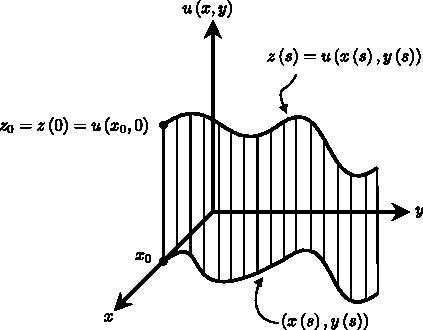
\includegraphics[width=0.35\paperwidth]{characteristics}
	\caption{The solution $u$ is described by the surface defined by
		$z=u\left(x,y\right)$.
		From any point $x_{0}$ on the $x$-axis, there is a curve
		$\left(x\left(s\right),y\left(s\right)\right)$ in the
		$xy$-plane, upon which wa can calculate the solution
		$z=u\left(x\left(s\right),y\left(s\right)\right)$.
		Knowing only the structure of the PDE, $x_{0}$ and $z_{0}$ we
		can solve ODEs to find the part of the solution surface which
		lies above the curve.}
\end{figure}

\begin{equation*}
	a\left(x,y\right)\diffp{u}{x}+
	b\left(x,y\right)\diffp{u}{y}=
	c_{1}\left(x,y\right)u+
	c_{2}\left(x,y\right),
	u\text{ given for }\left(x,y\right)\in\Gamma
\end{equation*}
where we have a linear PDE in the independent variables $x$ and $y$
with a given functions $a$, $b$, $c_{1}$ and $c_{2}$ of $\left(x,y\right)$.
$\Gamma\subset\partial\Omega$.
We find the characteristics, i.e., the curves which follow these directions, by solving
\begin{align*}
	\diff{x}{s}     & =
	a\left(x\left(s\right),y\left(s\right)\right). \\
	\diff{y}{s}     & =
	b\left(x\left(s\right),y\left(s\right)\right). \\
	z\left(s\right) & =
	u\left(x\left(s\right),y\left(s\right)\right).
\end{align*}

\begin{equation*}
	\diff{z}{s}=
	c_{1}\left(x\left(s\right),y\left(s\right)\right)
	z\left(s\right)+
	c_{2}\left(x\left(s\right),y\left(s\right)\right).
\end{equation*}

\section{Method of separation of variables}

\chapter{Code Repositories and Resources}

% \section{MOLE GitHub Repository}
% \section{Example Datasets} % TODO: Sparse matrices
% https://sci-hub.se/10.1137/S0895479801398025
